\documentclass[12pt,a4paper]{article}
\usepackage[utf8]{inputenc}
\usepackage[russian]{babel}
\usepackage[OT1]{fontenc}
\usepackage{amsmath}
\usepackage{amsfonts}
\usepackage{amssymb}
\usepackage{graphicx}
\graphicspath{{images/}}
\usepackage{wrapfig}
\usepackage[left=2cm,right=2cm,top=2cm,bottom=2cm]{geometry}
\usepackage{setspace}


\begin{document}

\title{
Отчет о выполнении лабораторной работы 1.2.3

Определение моментов инерции твердых тел с помощью трифилярного подвеса.
\author{Варламов Антоний, группа Б02-928}
}

\maketitle

\newpage

\textbf{Цель работы:} Измерение момента инерции тела и сравнение результатов с расчетами по теоретическим формулам. Проверка аддитивности моментов инерции и справедливости формулы Гюйгенса-Штейнера.

		
\textbf{В работе используются:} Трифилярный подвес (Рис. ~\ref{ris:trifilar}), секундомер, счетчик числа колебаний, набор тел, момент инерции которых необходимо измерить.

\section{Теоретические данные.}
	
	Перед началом работы кратко изложим теоретический материал,связанный с данной темой:
	\begin{wrapfigure}[10]{r}{0.5\textwidth}
   		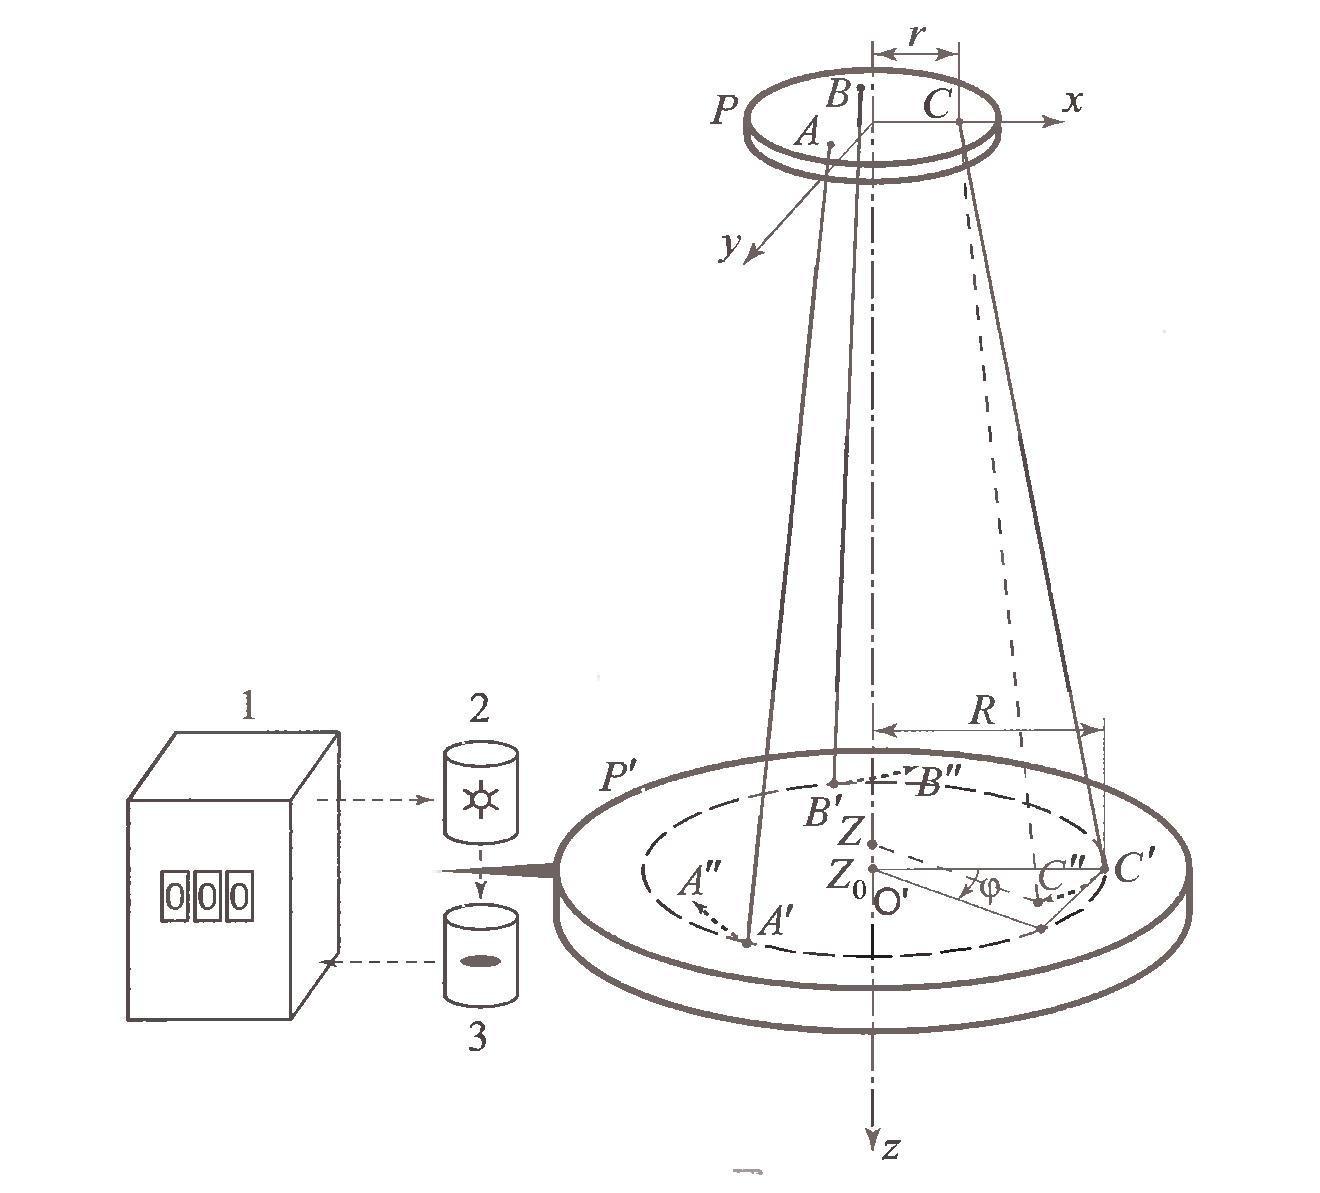
\includegraphics[width=0.4\textwidth]{schem_device}%
    	\caption{Трифилярный подвес}
    	\label{ris:trifilar}
	\end{wrapfigure}
	
	
	\begin{flushleft}
		\begin{spacing}{1.6}
		
			$ I = \int r^2 dm $
		
				
			$ \frac{I\ddot{\phi}^2}{2} + mg(z_{0} - z) = E $


			$ (R\cos\phi - r)^2 + R^2\sin^2\phi + z^2 = L^2 $

		
			$ z^2 = L^2 - R^2 - r^2 + 2Rr\cos\phi \approx z^2_{0} - 2Rr(1 - \cos\phi) \approx z^2_{0} - Rr\phi^2 $


			$ z = \sqrt{z^2_{0} - Rr\phi^2} \approx z_{0} - \frac{Rr\phi^2}{2z_{0}} $
			
		\end{spacing}
	\end{flushleft}
	
		Трифилярный подвес (Рис. ~\ref{ris:trifilar}) состоит из укрепленной на некоторой высоте 				неподвижной 	платформе P и подвешенной к ней на трех симмметрично расположенных нитях $ AA', BB', 		CC' $ вращающейся платформы P'.
	
		Подставляя данное уравнение в уравнение Закона Сохранения Энергии и дважды дифференцируя по 				времени, после сокращений, получаем:
		
	\begin{equation}
		 I\ddot{\phi}^2 + mg\frac{Rr}{z_{0}}\phi = 0 
		 \label{equ:first}	
	\end{equation}
	
	
		Решая уравнение (\ref{equ:first}) относительно $\phi$, получаем:
			
	
	\begin{equation}
		\phi = \phi_{0}\sin\left(\sqrt{\frac{mgRr}{Iz_{0}}}t + \theta\right)
		\label{equ:second}
	\end{equation}
	
	
	Из (\ref{equ:second}) следует, что 
	
	\begin{equation}
		T = 2\pi\sqrt{\frac{Iz_{0}}{mgRr}}		
	\end{equation}
	
	\begin{equation}
		I = kmT, \qquad k = \frac{gRr}{4\pi^2z_{0}} 
		\label{equ:four}
	\end{equation}

	\newpage	

\section{Выоплнение работы.}

	\subsection{Проверка установки.}
		
		\qquad  Перед началом выполнения лабораторной работы, выполним проверку установки. Для этого, возбудим крутильные колебания нижней платформы и определим время затухания. Установку будем считать исправной, если время затухания $$\tau \gg T$$
		
		Для удобства наблюдения, определим, за каrое время амплитуда колебаний платформы (угол $\alpha$ - угол отклонения от начального положения) уменьшиться в 2 раза.
		
		Для значения $\alpha \approx 45^{\circ}$ имеем: Время затухания: $\tau \approx 180$ секунд, $T \approx 1,5$ секунды. Соотношение выполняется, установка пригодна для проведения измерений. Кроме того, определим, при каком значении угла отклонения амплитуда практически независит от периода. Путем измерений начальное отклонение было выбрано $\alpha' \approx 30^{\circ}$
		
	\subsection{Определение параметров установки.}
	
		Работа выполнялась на установке №4, ее параметры занесены в таблицу \ref{tab:parametrs}
		\begin{table}[h!]
			\begin{center}
			\begin{tabular}{| l | l | l | l |}
					\hline
					m плат-мы, г & R, мм & r, мм & L, см \\ \hline
					934,7 & 114,6 & 30,5 & 216,2 \\
					\hline
				\end{tabular}
			\end{center} 
			\caption{Параметры установки.}
			\label{tab:parametrs}
		\end{table}
				
	\subsection{Определение момента инерции установки.}
	
		\qquad Для определения момента инерции установки возбудим крутильные колебания ненагруженной платформы. Измерим период колебаний ненагруженной платформы. Для этого измерим время $N$ полных колебаний установки. По результатам измерений определим $ T_{0} = \frac{N}{t}$.
		
		Результаты измерений: $ N = 50, t_{N} = 219.276$ cекунд
		
		 $T_{0} = 4,386$ c 
	\subsection{Определение момента инерции заданных тел. Проверка аддитивности момента инерции.}
	
		Определив период колебаний свободной платформы, можно перейти к определению периодов колебаний подвеса с грузами, установленными на платформе. Результаты измерений заносим в таблицу \ref{tab:periods_diff_body}.
		
		\begin{table}[ht!]
			\begin{center}
			\begin{tabular}{| p{65pt} | p{65pt} | p{55pt} | p{60pt}  | p{60pt} |}
					\hline
					Тело & Количество колебаний & Время колебаний, с & Период колебаний, с & Масса груза, г \\ \hline
					платформа & 50 & 219,276 & 4,386 & 934,7 \\ \hline
					платформа, кольцо & 50 & 212,796 & 4,256 & 1672,4 \\ \hline
					платформа, диск & 50 & 198,863 & 3,977 & 1520,3 \\ \hline
					платформа, кольцо, диск & 50 & 196,368 & 3, 927 & 2258 \\
					\hline
				\end{tabular}
			\end{center} 
			\caption{Периоды колебаний для различных тел на трифилярном подвесе.}
			\label{tab:periods_diff_body}
		\end{table}
		
		Для подтверждения аддитивности момента инерции необходимо показать, что выболняются соотношение:
		$$ I_{ring + disc} = I_{ring} + I_{disc} - I_{0} $$
		
		Для подтверждения данного соотношения вычислим соответсвующие моменты инерции, используя формулу (\ref{equ:four}). Результаты занесем в таблицу (\ref{tab:moments})
		
		\begin{table}[h!]
			\begin{center}
				\begin{tabular}{| l | c |}
				\hline
				Тело & Момент инерции, $kg*m^{2}, * 10^{-3}$ \\ \hline
				Платформа & 7,23 \\ \hline
				Платформа + диск & 9,67 \\ \hline
				Платформа + кольцо & 12,18 \\ \hline
				Платформа + диск + кольцо & 14,00 \\ \hline
				\end{tabular}
				\caption{Моменты инерции различных тел.}
				\label{tab:moments}
			\end{center}					
		\end{table}
		
		Подставляя эти данные в формулу $$ I_{ring + disc} = I_{ring} + I_{disc} - I_{0}, $$ получаем, что данное соотношение выполняется в пределах погрешности. Значит, доказано исходное предположение, \underline{момент инерции тела -- аддитивная величина}.
		\newpage
		
	\subsection{Определение зависимости момента инерции системы тел от их взаимного расположения.}
		\begin{wrapfigure}[10]{r}{0.29\textwidth}
			\vspace{-3em}
			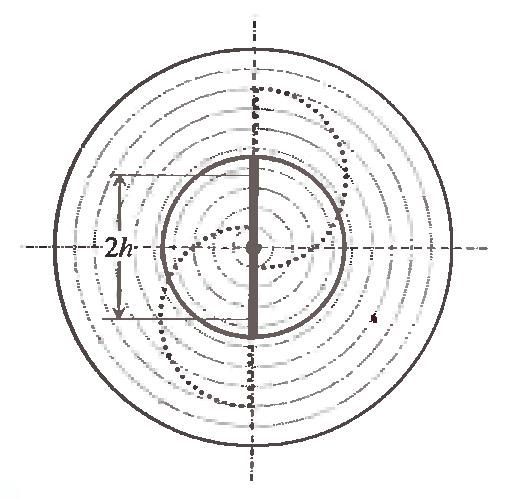
\includegraphics[width=0.25\textwidth]{position}
			\caption{Схема расположения грузов на платформе трифилярного подвеса.}
			\label{ris:position}
		\end{wrapfigure}
			
		Перрейдем к определению зависимости Момента инерции системы двух тел от их взаимного расположения. Для этого, располагая грузы как показано на рис. \ref{ris:position}, получим зависимость периода от расстояния. Затем, используя формулу (\ref{equ:four}), определим зависимость $ I(h^{2}) $
		
		Полученные результаты измерений занесем в таблицы \ref{tab:period},\ref{tab:moment} соответсвенно. Основывыаясь на результатах таблицы \ref{tab:moment}, построим график зависимости $ I(h^{2}) $. (Рис. \ref{ris:grafik})
		
		
		\begin{table}[b]
			\begin{center}
				\begin{tabular}{| l | l | l || l | l | l |}
					\hline
					№ изм. & T, с & h, сm & № изм. & T, с & h, сm \\ \hline
					1 & 3,122 & 0 & 8 & 3,399 & 3,5 \\ \hline
					2 & 3,127 & 0,5 & 9 & 3,472 & 4,0 \\ \hline
					3 & 3,146 & 1,0 & 10 & 3,568 & 4,5 \\ \hline
					4 & 3,167 & 1,5 & 11 & 3,662 & 5,0 \\ \hline
					5 & 3,207 & 2,0 & 12 & 3,753 & 5,5 \\ \hline
					6 & 3,255 & 2,5 & 13 & 3,886 & 6,0 \\ \hline
					7 & 3,325 & 3,0 & 14 & 4,002 & 6,5 \\ \hline
				\end{tabular}
				\caption{Зависимость Периода колебаний от расстояния между дисками.}
				\label{tab:period}
			\end{center}
		\end{table}
		
		\begin{table}[t]
			\begin{center}
				\begin{tabular}{| l | l | l || l | l | l |}
					\hline
					№ изм. & I, $kgm^2 * 10^{-3}$ & h, cm & № изм. & I, $kgm^2 * 10^{-3}$ & h, сm \\ \hline
					1 & 1,678 & 0 & 8 & 1,827 & 3,5 \\ \hline
					2 & 1,681 & 0,5 & 9 & 1,866 & 4,0 \\ \hline
					3 & 1,691 & 1,0 & 10 & 1,918 & 4,5 \\ \hline
					4 & 1,702 & 1,5 & 11 & 1,968 & 5,0 \\ \hline
					5 & 1,724 & 2,0 & 12 & 2,017 & 5,5 \\ \hline
					6 & 1,750 & 2,5 & 13 & 2,089 & 6,0 \\ \hline
					7 & 1,787 & 3,0 & 14 & 2,151 & 6,5 \\ \hline
				\end{tabular}
				\caption{Зависимость Момента инерции от расстояния между дисками.}
				\label{tab:moment}
			\end{center}
		\end{table}

		\begin{figure}
		

			\begin{center}
				\includegraphics[width=0.9\textwidth]{grafik}
				\caption{График зависимости $ I(h^2) $}
				\label{ris:grafik}
			\end{center}
		\end{figure}

		\newpage
		
	\subsection{Определение момента инерции диска, его массы.}
	
		
		Для определения момента инерции диска воспользуемся полученными в таблице \ref{tab:moment} значениями. Нас  интересует значение момента инерции при $ h = 0$. При таких условиях, $ I = 1,678 \times 10^{-3} \qquad kgm^2 $
		
		Определим, чему равна масса диска, используя формулу \ref{equ:four}:
		
		$ m = 1,348$г.
		
		Cравнивая результат с истинным значением, можно сказать, что отклонение полученного значения от истинного составляет $ 0,82 \% $.
		
	\subsection{Определение момента инерции тел, с использованием теоретических формул.}
		Определим, совпадают ли полученные значение моментов инерции с теоретическими.
		
		Для этого, используем следующие формулы:
		
		\newpage
		
		\begin{flushleft}
			\begin{spacing}{1.6}
				$ I_{disc} = \frac{1}{2}mR^2 $
				
				$ I_{ring} = mR^2 $
			\end{spacing}
		\end{flushleft}
		
		Подставив в данные формулы значения $ m $ и $ R $, получаем:		
		
		\begin{flushleft}
			\begin{spacing}{1.6}
				$ I_{disc teor} =  2,51 * 10^{-3} \quad kgm^2 $ 
				
				$ I_{ring teor} = 5,02 * 10^{-3} \quad kgm^2 $
			\end{spacing}
		\end{flushleft}	


		Данные результаты говорят о том, что измеренные таким образом моенты инерции практически не отличаются от теоретических данных.	 
	\subsection{Определение погрешностей измерений.}
		Необходимо определеить погрешности измеряемых величин, чтобы сказать, какой точности позволяет добиться метод. 
		Определим погрешность измерения $k : \sigma_{k}$
	
		\begin{flushleft}
			\begin{spacing}{1.6}
				$ \sigma_{k} = k\sqrt{\left(\frac{\sigma_{R}}{R}\right)^2 + \left(\frac{\sigma_{r}}{r}\right)^2 + \left(\frac{\sigma_{z_{0}}}{z_{0}}\right)^2} $
			
				$ \sigma_{k} = 0,01,\qquad k \approx 0,40$
			\end{spacing} 
		\end{flushleft}
		
		Определим относительную погрешность для измерения периода:
		\begin{flushleft}
			\begin{spacing}{1.6}
				$ \epsilon_{I} = \sqrt{\left(\frac{\sigma_{k}}{k}\right)^2 + 4\left(\frac{\sigma_{T}}{T}\right)^2} $
				$ \epsilon_{I} = 0,089 $
			\end{spacing} 
		\end{flushleft}
		 
		 Данный результат показывает, что с помощью данного метода можно определить момент инерции тела с точностью равной  $8,9\%$, при условии, что $\epsilon_{T} \approx 0,005$
		 
		\newpage		 
		 
\section{Вывод.}
	\begin{enumerate}
		\item Величина момента инерции, определенная с помощью трифилярного подвеса с довольно большой точностью совпадает с теоретическими предсказаниями. Большая точность обеспечивается малой погрешностью измерения времени, а также выбором условий, при которых крутильные колебания подвеса можно считать слабозатухающими.
		\item Была достигнута относительная точность определения момента инерции $ \epsilon_{I} = 0,089 $. Основной вклад в погрешность измерения момента инерции внесла погрешность косвенного измерения $z_{0}$. Данную погрешность можно уменьшить, если более точно определить параметры установки.
		\item Была полученая зависимость $ I(h^{2}) $. Данная зависимость довольно хорошо аппроксимируется линейной зависимость, что подтверждает теоретические данные.
		\item Была подтверждена аддитивность момента инерции.
	\end{enumerate}


\end{document}
